\section{Experimental Results}



    We evaluated the proposed approach on a dataset consisting of $N = 4$ books, two of which looking the same from the back.~\figref{fig:object_dataset} shows the covers of all the books used for the experiment. Each book was trained in $I = 4$ discrete poses being: cover up with visible spine, cover up with no visible spine, cover down with visible spine and cover down with no visible spine. All the poses are presented in~\figref{fig:pose_dataset}. For all object-pose pairs we extracted approximately $M = 654$ SIFT features which are later used for feature matching. We took $R = 100$ training images of each object-pose pair to learn the distribution $\prob{f|o,p}$. For the ambiguous case (the book looks the same from the cover down pose) we use the same training images amplify the ambiguity of the object recognition algorithm.

    Our experimental setup consists of a Microsoft Kinect sensor which we use as a RGB camera and one of the objects from the database. All the actions are executed by a human and we assume that there is no noise in the action execution. 

    \subsection{Object Recognition}
        In order to evaluate the object recognition part of the model, we compute average training and cross validation error for the dataset. For each object-pose pair we leave out 20 out 98 samples for the cross validation and we conduct training on the remaining 78 samples. The results are presented in~\tabref{tab:accuracy}. It is worth emphasizing that we did not include the cross validation results for ambiguous cases in the evaluation as the experiment is designed such that it confuses the object recognition algorithm (e.g. we use the same training images for the cover down poses).  
        
        \begin{table}[h]
                \centering
                \begin{tabular}{|c|c|}
                \hline
                Average Training Accuracy & Average Cross Validation Accuracy \\
                \hline
                99.67\% & 93.75\% \\
                \hline
                \end{tabular}
                \caption{Average accuracy results for object recognition part of the model.}
                \label{tab:accuracy}
        \end{table}

    \subsection{Action Selection}
        The experiment is constructed as follows. We expose an object to the Kinect sensor and obtain the recognition result. In the next step we employ the action selection algorithm to choose the best action and we execute it. In order to measure if the action improved the previous recognition we compute the posterior probability of the object.~\figref{fig:tree} presents a decision tree that is visualizes the best action actions chosen by the algorithm and the respective observations. The posterior probabilities of the object associated with the respective observation are shown in~\figref{fig:posteriors}. We execute actions until the algorithm converges which means that the action selection algorithm returns says that all the actions are equally informative.

    \subsection{Discussion}
    % describe the behaviour of posteriors
    % explain why it chose this action
    % explain why we took this exagurated example of the books with stickers
    % show encyclopedia example
    % talk a bit about continous pose    
        
\begin{figure}
            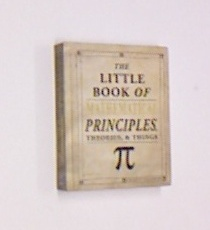
\includegraphics[width = 0.2\columnwidth]{pics/math_cover1_ok.jpg}
            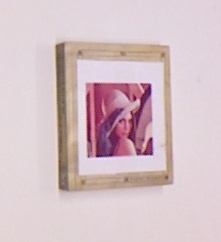
\includegraphics[width = 0.2\columnwidth]{pics/math_cover2_ok.jpg}
            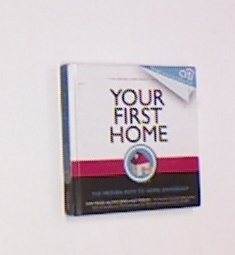
\includegraphics[width = 0.2\columnwidth]{pics/first_cover1.jpg}
            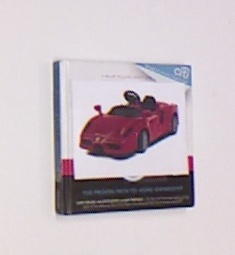
\includegraphics[width = 0.2\columnwidth]{pics/first_cover2.jpg}
            \caption{Books from the cover side used for the experiment. Two first books and two last books look the same from the back side.}
    \label{fig:object_dataset}
    \end{figure}        
        
        
    \begin{figure}
            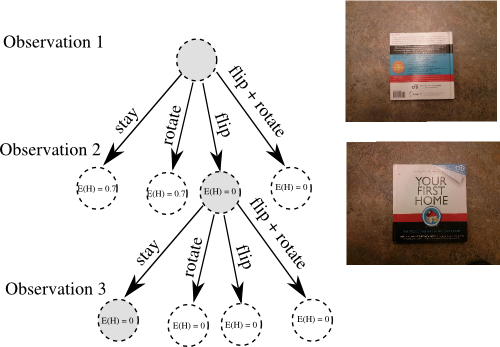
\includegraphics[width = \columnwidth]{pics/tree_small2.png}
        \label{fig:tree}
        \caption{Decision tree based on the action selection algorithm. Each node in the tree represents the expected entropy of the posterior probability for a given action. Colored nodes indicate the choice of the action that results in the minimum expected entropy. Directed edges correspond to all possible actions. Right: observed images for the observation before and after the action was taken . }
    \end{figure}
    
    \begin{figure}
            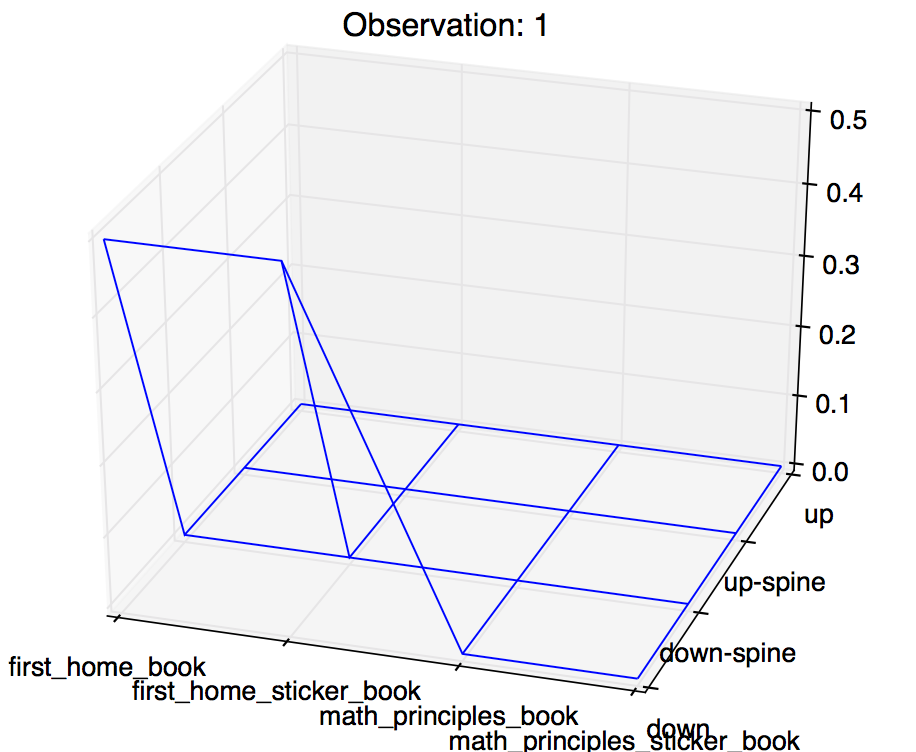
\includegraphics[width = \columnwidth]{pics/experimentObs1.png}
            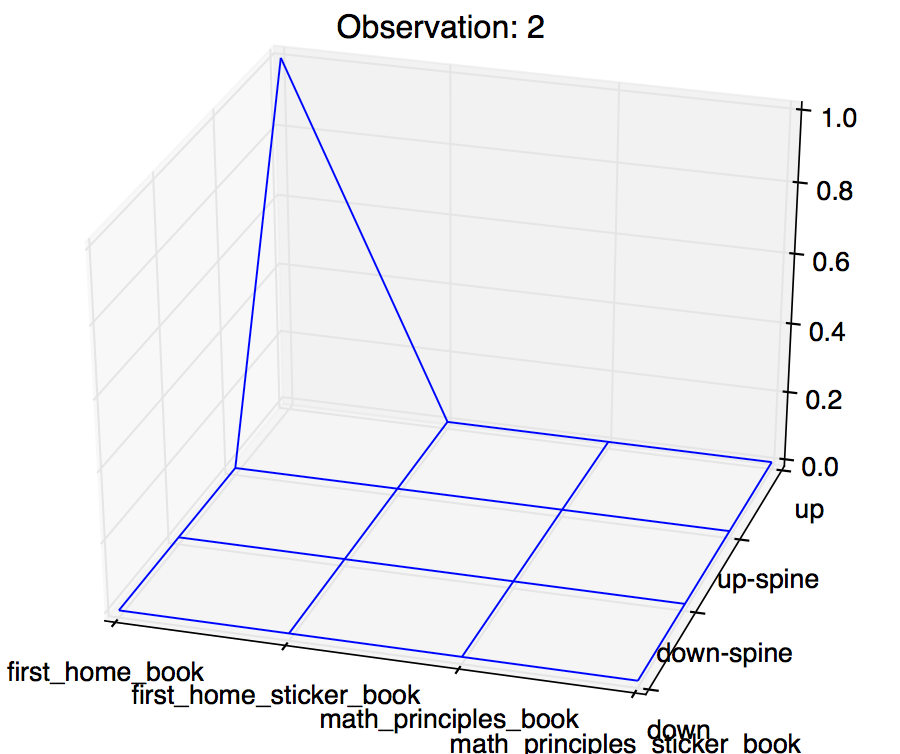
\includegraphics[width = \columnwidth]{pics/experimentObs2.png}
    \caption{Posterior probabilities of object and pose for the observations presented in~\figref{fig:tree}.}
        \label{fig:posteriors}
    \end{figure}
    
    
    
    %TODO: change picture of no spine images
     \begin{figure}
            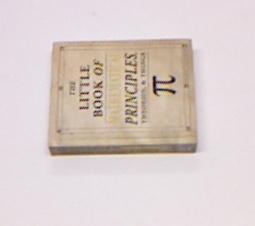
\includegraphics[width = 0.2\columnwidth]{pics/math_cover1.jpg}
            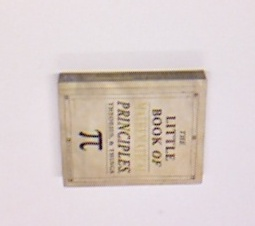
\includegraphics[width = 0.2\columnwidth]{pics/math_cover1_rot.jpg}
            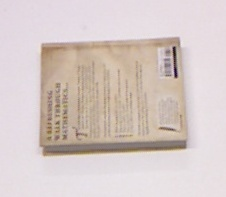
\includegraphics[width = 0.2\columnwidth]{pics/math_down.jpg}
            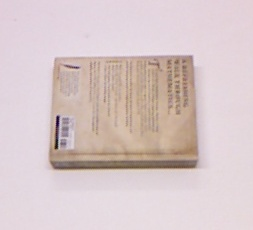
\includegraphics[width = 0.2\columnwidth]{pics/math_down_rot.jpg}
            \caption{All the poses that are used for object-pose recognition: cover up with visible spine, cover up with no visible spine, cover down with visible spine and cover down with no visible spine.}
    \label{fig:pose_dataset}
    \end{figure}
        
        


        %*explain our setup
        % we have a kinect, 4 object, 4 poses each, 50 sift features per object-pose pair
        % 100 training images per object-pose pair
        % we move the object with our hands for now
        %  

        %*assumptions
        % perfect actions (no noise)
        % discrete poses 
        % we see one object at a time
        % we see a known object

        %*explain experiment
        % we show the object to the kinect and recognize it based on our recognition module
        % results for all objects and poses are in the table
        % we figure out the best action (in the table)
        % we check recognition after the action has been taken (in the table)


%        \begin{itemize}
%        \item explain our dataset
%        \item show pictures of objects
%        \item show cross validation results for our training
%        \item explain the setup
%        \item show real data results for object recognition (table)
%        \item discuss the results, emphasize that the action selection works
%        \end{itemize}